


\documentclass{bredelebeamer}




%%%%%%%%%%%%%%%%%%%%%%%%%%%%%%%%%%%%%%%%%%%%%%%%



\graphicspath{{graphes/}}

\title[MEMO-F508]{Test d'ordonnançabilité pour systèmes à criticité mixte\\par exploration d'automates}
% Titre du diaporama

\subtitle{MEMO-F508 -- Masters thesis}



\author{Simon \textsc{Picard}}
% La commande \inst{...} Permet d'afficher l' affiliation de l'intervenant.
% Si il y a plusieurs intervenants: Marcel Dupont\inst{1}, Roger Durand\inst{2}
% Il suffit alors d'ajouter un autre institut sur le modèle ci-dessous.

\institute[ULB]
{
  \textsc{Université libre de Bruxelles}\\
  Faculté des Sciences\\
  Département d'Informatique
  }


\date{17 Juin 2016}
% Optionnel. La date, généralement celle du jour de la conférence

\subject{Ordonnancement criticité mixte et techniques de vérifications formelles}
% C'est utilisé dans les métadonnes du PDF




%%%%%%%%%%%%%%%%%%%%%%%%%%%%%%%%%%%%%%%%%%%%%%%%%%%%%%%%%%%%%%%%%%%%%
\begin{document}

\begin{frame}
  \titlepage
\end{frame}





\begin{frame}{Sommaire}
  \tableofcontents
\end{frame}



\section[Criticité mixte]{Ordonnancement en criticité mixte}

\begin{frame}{Ordonnancement en criticité mixte}

\begin{itemize}
\item Partager une ou plusieurs ressources entre plusieurs entités
\item Temps réel : contraintes temporelles
\item Notion de criticité
\item Représentation sous forme de travaux $J_i = (r_i, d_i, \chi_i, c_i)$
\item Plusieurs temps d'exécution
\item Considérer deux niveaux de criticité, haut et bas, faible et fort
\end{itemize}

\end{frame}

\begin{frame}{Ordonnancement en criticité mixte}

\begin{exampleblock}{Faisabilité CM}
Il est possible d'agencer les travaux correctement \begin{itemize}
\item $\forall \ell, \forall J_i : \chi_i \geq \ell \rightarrow $ exécution jusqu'à complétion durant $[r_i, d_i)$
\end{itemize}
\end{exampleblock}

\begin{block}{Ordonnançabilité CM}
Il existe un algorithme en ligne qui permet d'ordonnancer correctement les travaux\begin{itemize}
\item Complexe car en ligne
\item Problème NP-difficile
\end{itemize}
\end{block}



\end{frame}

\begin{frame}{Test d'ordonnançabilité}

Si un test d'ordonnançabilité échoue, il peut y avoir différentes raisons
\begin{exampleblock}{Faisabilité}
Le système en tant que tel n'est pas faisable.
\begin{itemize}
\item Testable par condition sur utilisation
\end{itemize}
\end{exampleblock}

\begin{block}{Ordonnançabilité}
Le système n'est pas ordonnançable.
\end{block}

\begin{alertblock}{Test}
Le test est mal fait.
\end{alertblock}

\begin{itemize}
\item Deux derniers cas indissociables actuellement
\item Solution : tester tous les ordonnancements possibles
\item Réduction vers le problème d'accessibilité
\end{itemize}



\end{frame}

\section[Accessibilité]{Accessibilité dans un automate}

\begin{frame}{Problème d'accessibilité}

\begin{columns}

\begin{column}{0.5\textwidth}
\begin{itemize}
\item Graphe, sommets et arcs
\item Automates finis, ensemble de départ et d'arrivée
\item Chemin, séquence d'état adjacent
\end{itemize}
\end{column}
\begin{column}{0.45\textwidth}
\begin{figure}
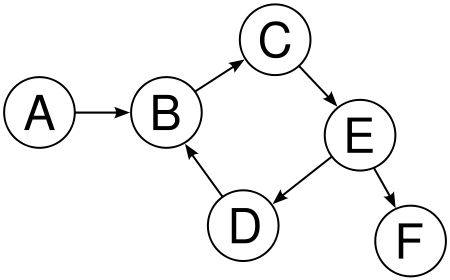
\includegraphics[scale = 0.3]{images/dgraph.png}
\caption{Exemple de graphe}
\end{figure}
\end{column}

\end{columns}


\begin{block}{États accessibles}
\centering
$Reach(A) = \{v \in V | \exists\ un\ chemin\ v_1,...,v_t : v_1 \in S_0 \wedge v_t = v\}$
\end{block}


\begin{itemize}
\item États d'arrivée $\cap$ États accessibles $\stackrel{?}{=} \emptyset$
\item Recherche en largeur
\item Linéaire en la taille de l'automate
\end{itemize}


\end{frame}

\begin{frame}{Antichaîne}

\begin{block}{Relation de simulation}
Soit $A = (V,E,S_0,F)$ un automate fini, un préordre $\succeq$ sur $V$ est une relation de simulation\index{relation de simulation} pour $A$ si:
\begin{itemize}

\item Pour tout $v_1, v_2, v_3 \in V$, si $v_2 \succeq v_1$ et $(v_1, v_3) \in E$, alors il existe $v_4 \in V$ tel que $v_4 \succeq v_3$ et $(v_2, v_4) \in E$.
\item Pour tout $v_1, v_2 \in V$, si $v_2 \succeq v_1 : v_1 \in F$ implique $v_2 \in F$.


\end{itemize}
\end{block}
\begin{figure}
\centering
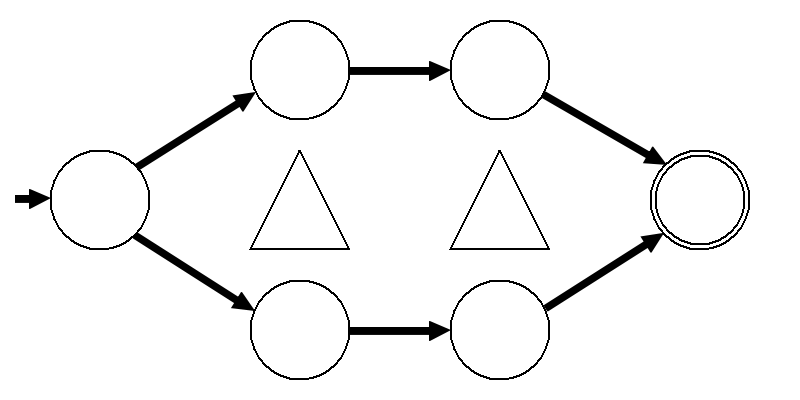
\includegraphics[scale=0.30]{images/exanti2.png}
\end{figure}


\begin{block}{Antichaîne}
\centering
$H = \{v_1 \in V|\forall v_2 \in V : v_1 \succeq v_2 \Rightarrow v_1 = v_2\}$
\end{block}
\end{frame}


\section[Test]{Algorithme d’ordonnancement}

\begin{frame}{Vestal \& AMC-max}
\begin{block}{Vestal}
\begin{itemize}
\item Basé sur Audsley
\item Tâche éligible à recevoir la plus faible priorité
\item Pire temps de réponse
\item Taille maximale de l'intervalle compris entre la génération d’un travail et sa complétion
\item Doit être inférieur à l'échéance
\end{itemize}
\end{block}

\begin{block}{AMC-max}
Décomposé le pire temps de réponse
\begin{itemize}
\item Temps en basse criticité
\item Temps en haute criticité
\item Temps durant le changement de criticité
\end{itemize}
\end{block}

Si l'assignation de priorité existe, alors le système est ordonnançable.

\end{frame}


\begin{frame}{OCBP}

\begin{block}{Algorithme}
\begin{itemize}
\item Audsley sur travaux
\item Assigner des priorité durant une période occupé
\item Considéré les travaux comme généré au plus tôt
\item Si premption d'un travail car émission d'un autre plus prioritaire, recalculer les priorité
\end{itemize}
\end{block}

\begin{block}{Test}
\begin{itemize}
\item Test basé sur la charge de travail
\item Portion de la capacité d’exécution requise pour respecter toutes les échéances
\end{itemize}
\end{block}

\end{frame}


\begin{frame}{PLRS \& LPA}

\begin{block}{PLRS}
\begin{itemize}
\item Crée une assignation de priorité pour les travaux
\item Ajuste au vol les priorité, en minimisant le nombre de calcul
\item Nécéssite de calculer la taille de plus grange période occupée
\end{itemize}
Si l'assignation initiale existe, le système de tâche est ordonnançable.
\end{block}

\begin{block}{LPA}
\begin{itemize}
\item PLRS en utilisant une taille de la période occupé mieux bornée
\end{itemize}
Si l'assignation initiale existe, le système de tâche est ordonnançable.
\end{block}

\end{frame}


\begin{frame}{EDF-VD \& Greedy}

\begin{block}{EDF-VD}

\begin{itemize}
\item Utiliser EDF en modifiant les échéance des tâche fortement critique, durant le niveau de criticité plus faible.
\item Test sur utilisation.
\end{itemize}
\end{block}


\begin{block}{Greedy}
\begin{itemize}
\item Utiliser EDF en modifiant les échéance.
\item Test sur fonction de borne de demande et d'approvisionement
\begin{itemize}
\item Fonction de borne de demande en faible criticité
\item Fonction de borne de demande en haute criticité
\item Travaux transféré
\end{itemize}
\item Heurisitique pour trouver les nouvelles échéance.
\end{itemize}
\end{block}

\end{frame}


\begin{frame}{LWLF}

\begin{itemize}
\item Basé sur LLF
\item Pire laxité, laxité pour un travail dans le pire des cas, pour son pire WCET.
\item Le travail ayant la plus petite pire laxité est ordonnancé.
\end{itemize}

\end{frame}

\section[Réduction]{Sémantique sous forme d'automate}

\begin{frame}{Périodique}
\begin{block}{Etat du système}
Soit $\tau = \tau_1, \tau_2, \tau_3 ...$ un système de tâches CM périodiques, l'état du système\index{automate périodique!etat du système@état du système} de $\tau$ est le tuple $S \overset{def}{=} \langle at_S, rct_S, crit_S\rangle$ avec
\begin{itemize}
\item $at_S$, une fonction représentant le temps d'arrivée du travail CM courant d'une tâche CM : $\tau \rightarrow \mathbb{N},\ at_S(\tau_i) \leq R_{max}$ avec $R_{max} \overset{def}{=} max(max_i\ (T_i),\ max_i\ (O_i))$
\item $rct_S$, le temps de calcul restant du travail CM généré par une tâche CM : $ \tau \rightarrow \mathbb{N},\ 0 \leq rct_S(\tau_i) \leq C_{max}$ avec $C_{max} \overset{def}{=} max_{i,j}\ C_i(j)$
\item $crit_S$, le niveau de criticité actuel du scénario, $ \in \mathbb{N},\ 1 \leq crit_S \leq K$\\
\end{itemize}
\end{block}

\begin{block}{Transitions}
\begin{itemize}
\item Transition d'exécution.
\item Transition de terminaison.
\item Transition critique.
\end{itemize}
\end{block}
\end{frame}


\begin{frame}{Sporadique}

\begin{block}{Etat du système}
Soit $\tau = \tau_1, \tau_2, \tau_3 ...$ un système de tâches CM sporadiques, l'état du système\index{automate sporadique!etat du systeme@état du système} de $\tau$ est le tuple $S \overset{def}{=} \langle nat_S, rct_S, done_S, crit_S \rangle$ avec

\begin{itemize}
\item $nat_S$, une fonction représentant le temps d'arrivée minimum du prochain travail CM d'une tâche CM : $\tau \rightarrow \mathbb{N},\ nat_S(\tau_i) \leq R_{max}$ avec $R_{max} \overset{def}{=} max(max_i\ (T_i),\ max_i\ (O_i))$
\item $rct_S$, le temps de calcul restant du travail CM généré par une tâche CM : $ \tau \rightarrow \mathbb{N},\ 0 \leq rct_S(\tau_i) \leq C_{max}$ avec $C_{max} \overset{def}{=} max_{i,j}\ C_i(j)$
\item $done_S$, la complétion d'un travail CM : $ \tau \rightarrow \{True,False\}$
\item $crit_S$, le niveau de criticité actuel du scénario, $ \in \mathbb{N},\ 1 \leq crit_S \leq K$\\
\end{itemize}
\end{block}

\begin{block}{}
\begin{columns}
\begin{column}{0.6\textwidth}
\begin{itemize}
\item Tâches CM actives, oisives et abandonnées
\item Tâches CM implicitement terminées
\item Tâches CM éligible à la soumission d'un travail
\end{itemize}
\end{column}
\begin{column}{0.4\textwidth}
\begin{itemize}
\item Criticité réelle d'un état
\item Laxité, pire laxité et états erronés
\item Ordonnanceur
\end{itemize}
\end{column}
\end{columns}
\end{block}

\end{frame}


\begin{frame}{Transition d'exécution}
Soit $S = \langle nat_S, rct_S, done_S, crit_S \rangle$ un état du système et $Run$ un \textit{ordonnanceur} pour $\tau$. On dit que l'état du système $S^+ = \langle nat_S^+, rct_S^+, done_S^+, crit_S^+ \rangle$ est un \textit{successeur-exécuté} de $S$ avec $Run$, noté $S\xrightarrow{Run}S^+$, si et seulement si:
\begin{itemize}
\item Pour tout $\tau_i \in Run(S) : rct_S^+(\tau_i) = rct_S(\tau_i)-1$
\item Pour tout $\tau_i \not \in Run(S) : rct_S^+(\tau_i) = rct_S(\tau_i)$
\item Pour tout $\tau_i \in \tau :$
$$ nat_S^+(\tau_i) = \left\{
    \begin{array}{ll}
        max(nat_S(\tau_i)-1, 0) & si\ \tau_i \notin Active(S) \\
        nat_S(\tau_i)-1 & si\ \tau_i \in Active(S) 
    \end{array}
\right.
$$
\item $done_{S}^{+} = done_{S}$
\item $crit_{S}^{+} = crit_{S}$\\
\end{itemize}
\end{frame}


\begin{frame}{Transition de terminaison}
Soit $S = \langle nat_S, rct_S, done_S, crit_S\rangle$ un état du système et $\tau^T \subseteq Active(S)$ un ensemble de tâches CM actives pouvant signaler leur complétion. On dit que l'état du système $S^T = \langle nat_S^T, rct_S^T, done_S^T, crit_S^T \rangle$ est un \textit{successeur-$\tau^T$-terminé} de $S$, noté $S\xrightarrow{\tau^T}S^T$, si et seulement si:

\begin{itemize}
\item Pour tout $\tau_i \in \tau^T \cup ImplicitelyDone(S)$ :\begin{itemize}
\item $rct_{S}^T(\tau_i) = 0$
\item $done_{S}^T(\tau_i) = True$
\end{itemize}
\item Pour tout $\tau_i\ \notin \tau^T \cup ImplicitelyDone(S)$ :\begin{itemize}
\item $rct_{S}^T(\tau_i) = rct_{S}(\tau_i)$
\item $done_{S}^T(\tau_i) = done_{S}(\tau_i)$
\end{itemize}
\item $nat_{S}^T = nat_{S}$
\item $crit_{S}^T = crit_{S}$\\
\end{itemize}
\end{frame}


\begin{frame}{Transition critique}
Soit $S = \langle nat_S, rct_S, done_S, crit_S \rangle$ un état du système. On dit que l'état du système $S^C = \langle nat_S^C, rct_S^C, done_S^C, crit_S^C \rangle$ est un \textit{successeur-critique} de $S$, noté $S\xrightarrow{C}S^C$, si et seulement si :

\begin{itemize}
\item $crit_S^C = Critical_S$
\item Pour tout $\tau_i \in \tau :$

\noindent $$
\begin{array}{rl}
rct_S^C(\tau_i) =  &\left\{
    \begin{array}{ll}
        rct_S(\tau_i)+c_i(Critical_S)-c_i(crit_S) & si\ X_i\geq Critical_S \wedge \tau_i \in Active(S)\\
        rct_S(\tau_i) & si\ X_i\geq Critical_S \wedge \tau_i \notin Active(S)\\
        0 & \mbox{sinon.}
    \end{array}
\right.\\
 nat_S^C(\tau_i) = &\left\{
    \begin{array}{ll}
        nat_S(\tau_i) & si\ X_i\geq Critical_S \\
        0 & \mbox{sinon.}
    \end{array}
\right.\\
 done_S^C(\tau_i) = &\left\{
    \begin{array}{ll}
        done_S(\tau_i) & si\ X_i\geq Critical_S \\
        True & \mbox{sinon.}
    \end{array}
\right.
\end{array}
$$
\end{itemize}
\end{frame}


\begin{frame}{Transition de requête}
Soit $S = \langle nat_S, rct_S, done_S, crit_S \rangle$ un état du système et $\tau^R \subseteq Eligible(S)$ un ensemble de tâches CM éligibles. On dit que l'état du système $S^R = \langle nat_S^R, rct_S^R, done_S^R, crit_S^R \rangle$ est un \textit{successeur-$\tau^R$-requête} de $S$, noté $S\xrightarrow{\tau^R}S^R$, si et seulement :
\begin{itemize}
\item Pour tout $\tau_i \in \tau^R$ :\begin{itemize}
    \item $nat_S(\tau_i)+T_i \leq nat_S^R(\tau_i) \leq T_i$
    \item $rct_S^R(\tau_i)=C_i(crit_S)$
    \item $done_S^R(\tau_i) = False$
\end{itemize}
\item Pour tout $\tau_i\ \notin \tau^R$ :\begin{itemize}
    \item $nat_S^R(\tau_i)=nat_S(\tau_i)$
    \item $rct_S^R(\tau_i)=rct_S(\tau_i)$
    \item $done_S^R(\tau_i) = done_S(\tau_i)$
\end{itemize}
\item $crit_S^R = crit_S$\\
\end{itemize}
\end{frame}

\begin{frame}{Automate}
Étant donné un système de tâches CM sporadiques $\tau$ et un ordonnanceur $Run$, l'automate $\overline{A}(\tau,Run)$ est le tuple $(V, E, S_0, F)$ où:
\begin{itemize}
\item  $V=States(\tau)$
\item $(S_1,S_2) \in E$, si et seulement s'il existe les états intermédiaires $S^{+}, S^{T}$ et $S^{C} \in States(\tau)$ et $\tau^T \subseteq Run(S_1),\tau^R \subseteq Eligilbe(S^{C}) $ tel que : \\$S_1\xrightarrow{Run}S^{+}\xrightarrow{\tau^T}S^{T}\xrightarrow{C}S^{C}\xrightarrow{\tau^R}S_2$
\item $S_0 = (nat_{S_0}, rct_{S_0}, done_{S_0}, crit_{S_0})$ :\begin{itemize}
\item $nat_{S_0}(\tau_i) = O_i\ \forall\ i$
\item $rct_{S_0}(\tau_i) = 0\ \forall\ i$
\item $done_{S_0}(\tau_i) = True\ \forall\ i$
\item $crit_{S_0} = 1$
\end{itemize}
\item $F = Fail_\tau$
\end{itemize}
\end{frame}

\begin{frame}{Exemple I}
\centering
\begin{tabular}{|c|c|c|c|c|c|}
\hline
i &O & T & D & C & $\chi$\\
\hline
0 & 0 & 3 & 3 & [2, 3]& 2\\
\hline
\end{tabular}
\begin{figure}[h]
    \centering
    \resizebox{\textwidth-1cm}{!}{
    \fontsize{28pt}{12pt}\selectfont
    \input{graphes/spo-inter-1.pdf_tex}
    }
\end{figure}
\end{frame}

\begin{frame}{Exemple II}
\centering
\begin{tabular}{|c|c|c|c|c|c|}
\hline
i &O & T & D & C & $\chi$\\
\hline
0 & 0 & 3 & 3 & [2, 3]& 2\\
\hline
\end{tabular}
\begin{figure}[h]
    \centering
    \resizebox{\textwidth-1cm}{!}{
    \fontsize{28pt}{12pt}\selectfont
    \input{graphes/spo-inter-2.pdf_tex}
    }
\end{figure}

\end{frame}

\begin{frame}{Exemple III}
\centering
\begin{tabular}{|c|c|c|c|c|c|}
\hline
i &O & T & D & C & $\chi$\\
\hline
0 & 0 & 3 & 3 & [2, 3]& 2\\
\hline
\end{tabular}
\begin{figure}[h]
    \centering
    \resizebox{\textwidth-1cm}{!}{
    \fontsize{28pt}{12pt}\selectfont
    \input{graphes/spo-concat.pdf_tex}
    }
\end{figure}

\end{frame}


\begin{frame}{Simulation de tâche oisive}
Soit $\tau$ un système de tâches CM sporadiques. Le préordre de tâches oisives\index{simulation de tâches oisives} $\succeq_{idle} \subseteq States(\tau)\times States(\tau)$ est tel que pour tout $S_1, S_2 : S_2 \succeq_{idle}S_1$, si et seulement si :
\begin{itemize}
\item $crit_{S_2} = crit_{S_1}$
\item $done_{S_2} = done_{S_1}$
\item $rct_{S_2} = rct_{S_1}$
\item Pour tout $\tau_i$ tel que $done_{S_1}(\tau_i) = True : nat_{S_2}(\tau_i) \leq nat_{S_1}(\tau_i)$
\item Pour tout $\tau_i$ tel que $done_{S_1}(\tau_i) = False : nat_{S_2}(\tau_i) = nat_{S_1}(\tau_i)$\\
\end{itemize}
\end{frame}

\begin{frame}{Exemple}
\centering
\begin{tabular}{|c|c|c|c|c|c|}
\hline
i &O & T & D & C & $\chi$\\
\hline
0 & 0 & 2 & 3 & [1, 2]& 2\\
\hline
0 & 0 & 1 & 1 & [1, 1]& 1\\
\hline
\end{tabular}
\begin{figure}[h]
\centering
    \resizebox{\textwidth-2cm}{!}{
    \fontsize{28pt}{12pt}\selectfont
\input{graphes/idle-fail.pdf_tex}
}
\label{idle:exem:fail}

\end{figure} 
\end{frame}

\section{Résultats}


\begin{frame}{Méthodologie}
\begin{block}{}

Un système de tâches CM à double criticité est généré en commençant avec un ensemble vide $\tau = \emptyset$ dans lequel des tâches CM aléatoires sont ajoutées.
\begin{itemize}
\item la probabilité $P_{HI}$ que la tâche CM soit fortement critique
\item le ratio maximum $R_{HI}$ entre le temps d'exécution pour forte criticité et faible criticité
\item et la période maximum $T^{MAX}$
\end{itemize}

\end{block}

1500 systèmes de tâches CM ont été générés avec 2, 3 ou 4 tâches CM par ensemble


\end{frame}

\begin{frame}{Sporadique : avec antichaîne vs sans antichaîne}

\begin{figure}[h]
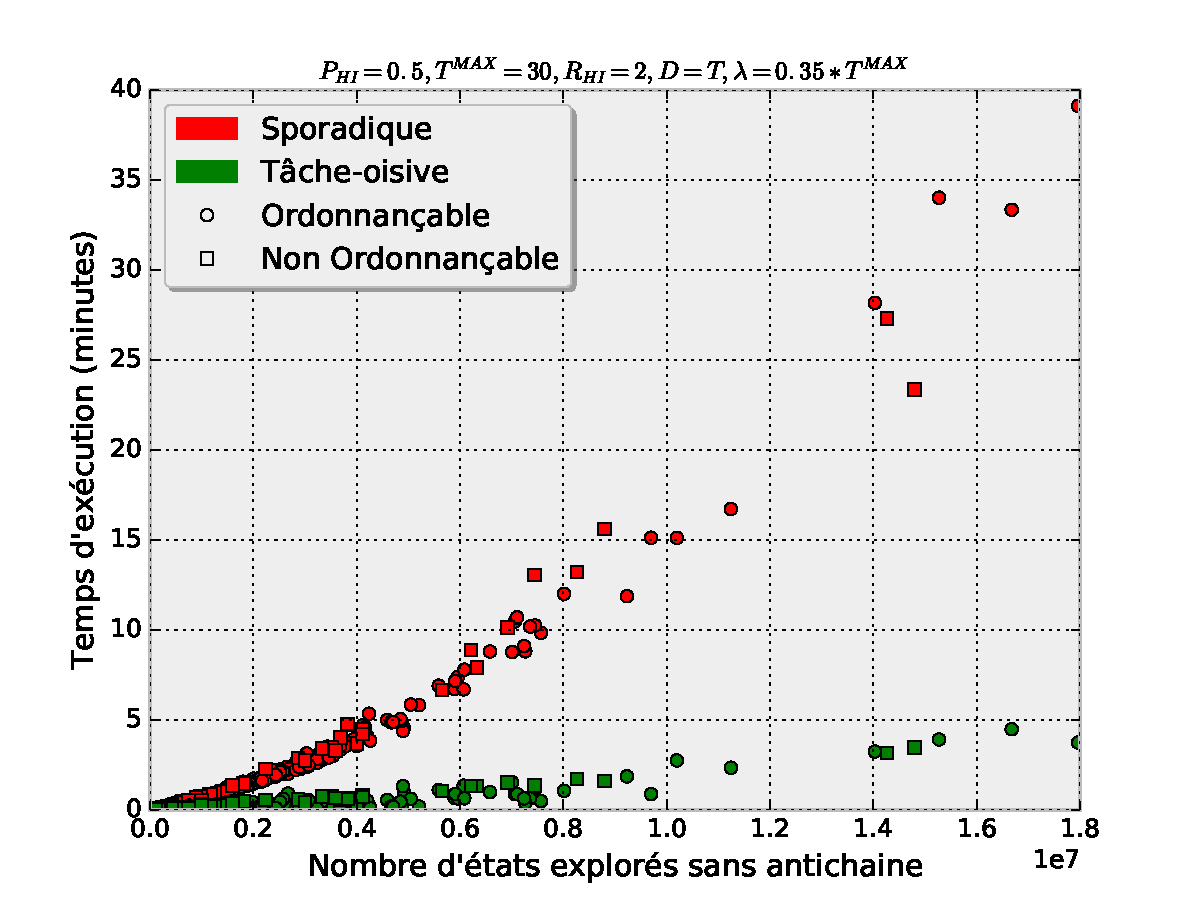
\includegraphics[width=\textwidth,height=0.8\textheight,keepaspectratio]{./results/timeSpoIdle.pdf}
\caption{Analyse de la performance de la relation de simulation}
\label{res:spoIdle}

\end{figure}

\end{frame}


\begin{frame}{Périodique vs sporadique avec antichaîne}

\begin{figure}[h]
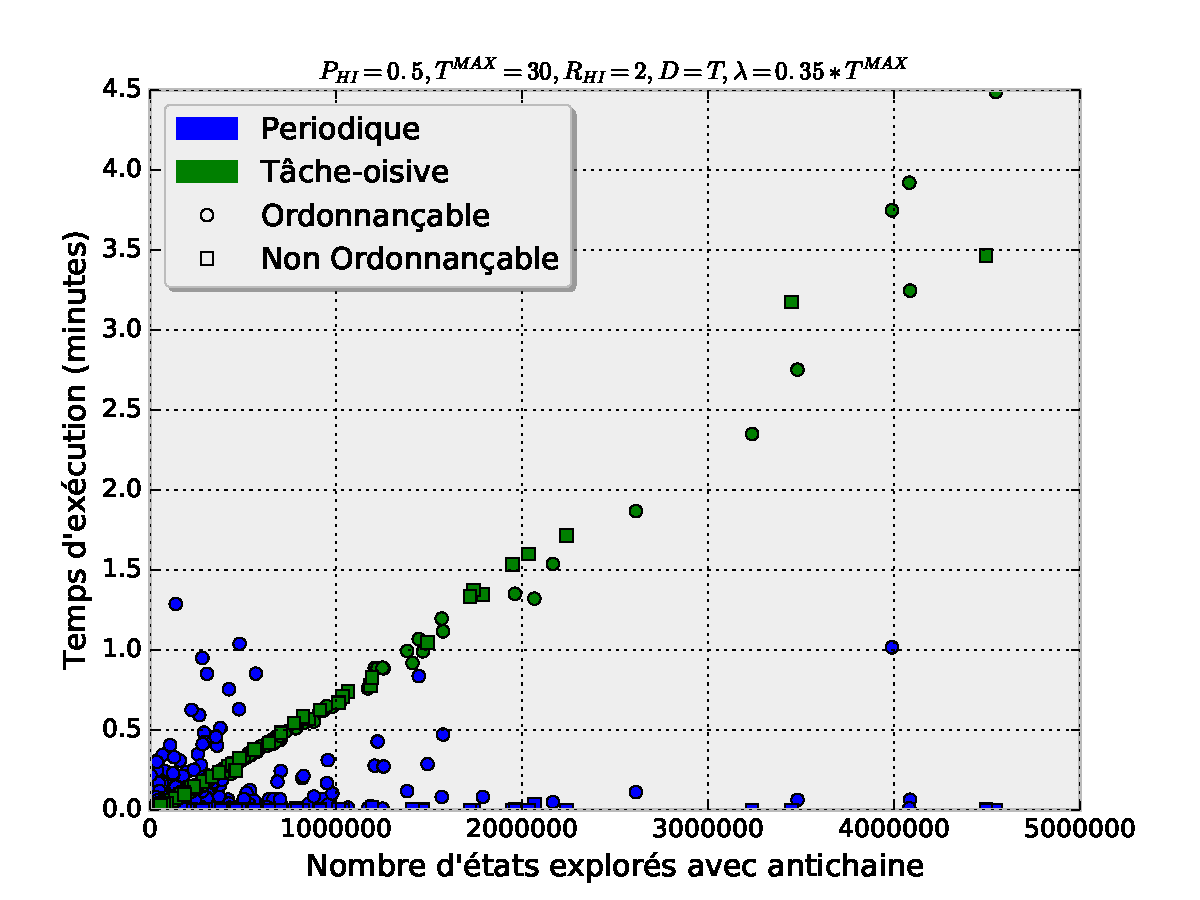
\includegraphics[width=\textwidth,height=0.8\textheight,keepaspectratio]{./results/timePerIdle.pdf}
\caption{Analyse de la performance de la relation de simulation}
\label{res:per-idle}
\end{figure}

\end{frame}


\begin{frame}{Complexité en espace}
\begin{figure}[h]
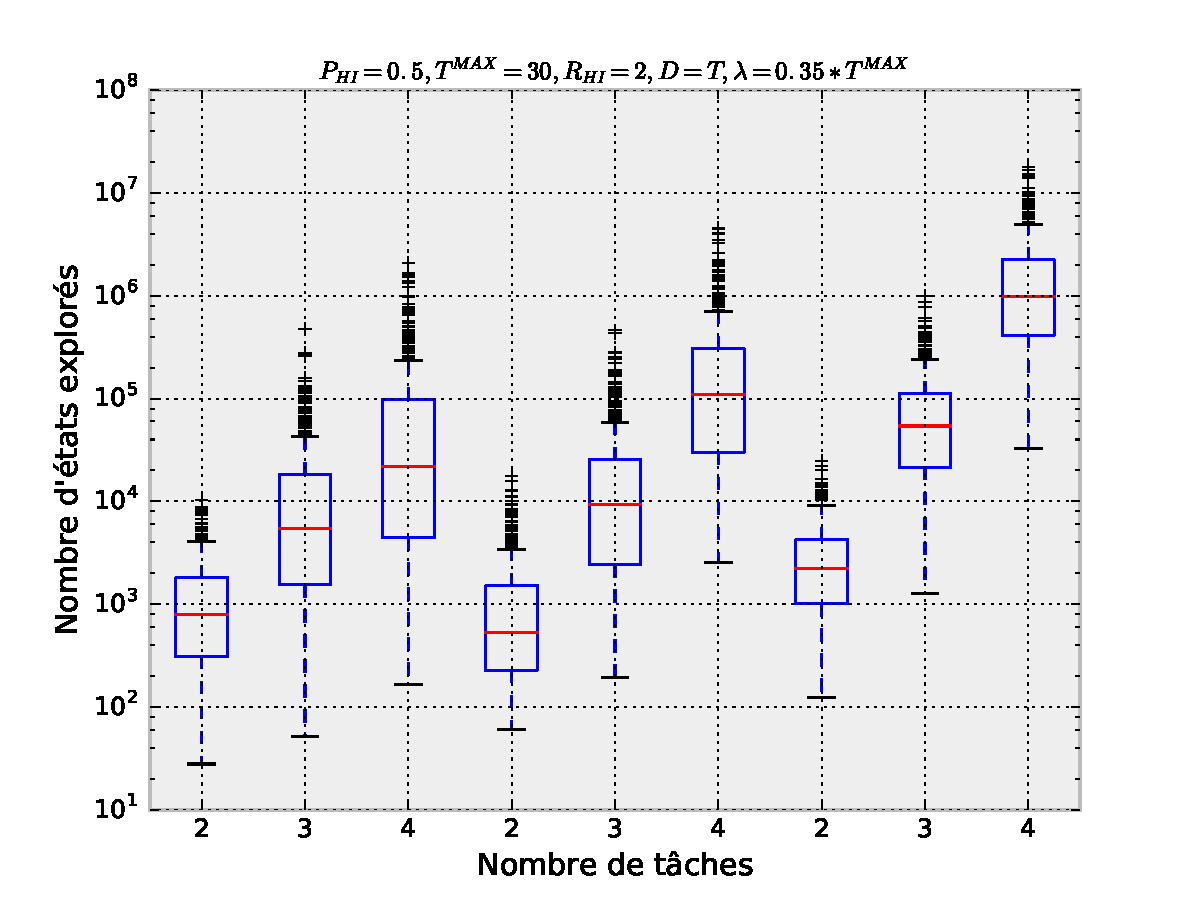
\includegraphics[width=\textwidth,height=0.8\textheight,keepaspectratio]{./results/taskvssize.pdf}
\caption{Taille de l'automate en fonction du nombre de tâches CM}
\label{res:nbetat}
\end{figure}
\end{frame}


\begin{frame}{Méthodologie}
\begin{block}{}

Un système de tâches CM à double criticité est généré en commençant avec un ensemble vide $\tau = \emptyset$ dans lequel des tâches CM aléatoires sont ajoutées. La génération des tâches CM est contrôlée par quatre paramètres :
\begin{itemize}
\item la probabilité $P_{HI}$ que la tâche CM soit fortement critique
\item le ratio maximum $R_{HI}$ entre le temps d'exécution pour forte criticité et faible criticité
\item et la période maximum $T^{MAX}$
\item $C^{MAX}_{LO}$, le temps d'exécution maximum pour faible criticité
\item utilisation moyenne objective $U^{*'}$
\end{itemize}

\end{block}

\begin{itemize}
\item $U^{*'}$ = $0.4 + (x/40) * 0.6$ pour $0 \le x \le 40$
\item Taux sur 2000 simulations
\item 4 tâches par systèmes
\end{itemize}


\end{frame}


\begin{frame}{Vestal vs AMC-max}
\begin{figure}[h]
\centering
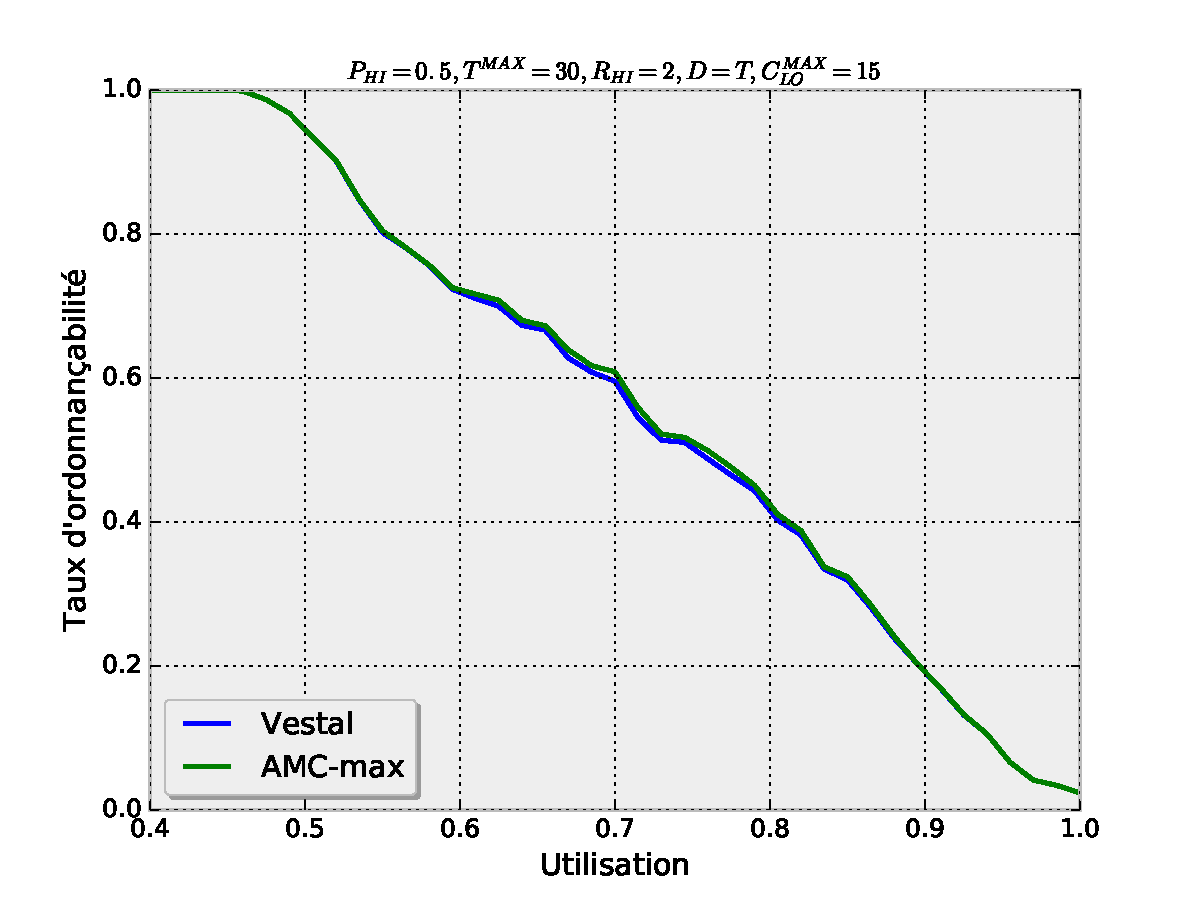
\includegraphics[width=\textwidth,height=0.8\textheight,keepaspectratio]{./results/perfAMCVestal.pdf}
\caption{Ordonnançabilité de Vestal et AMC-max}
\label{res:vestalamc}
\end{figure}
\end{frame}


\begin{frame}{OCBP, PLRS \& LPA}
\begin{figure}[h]
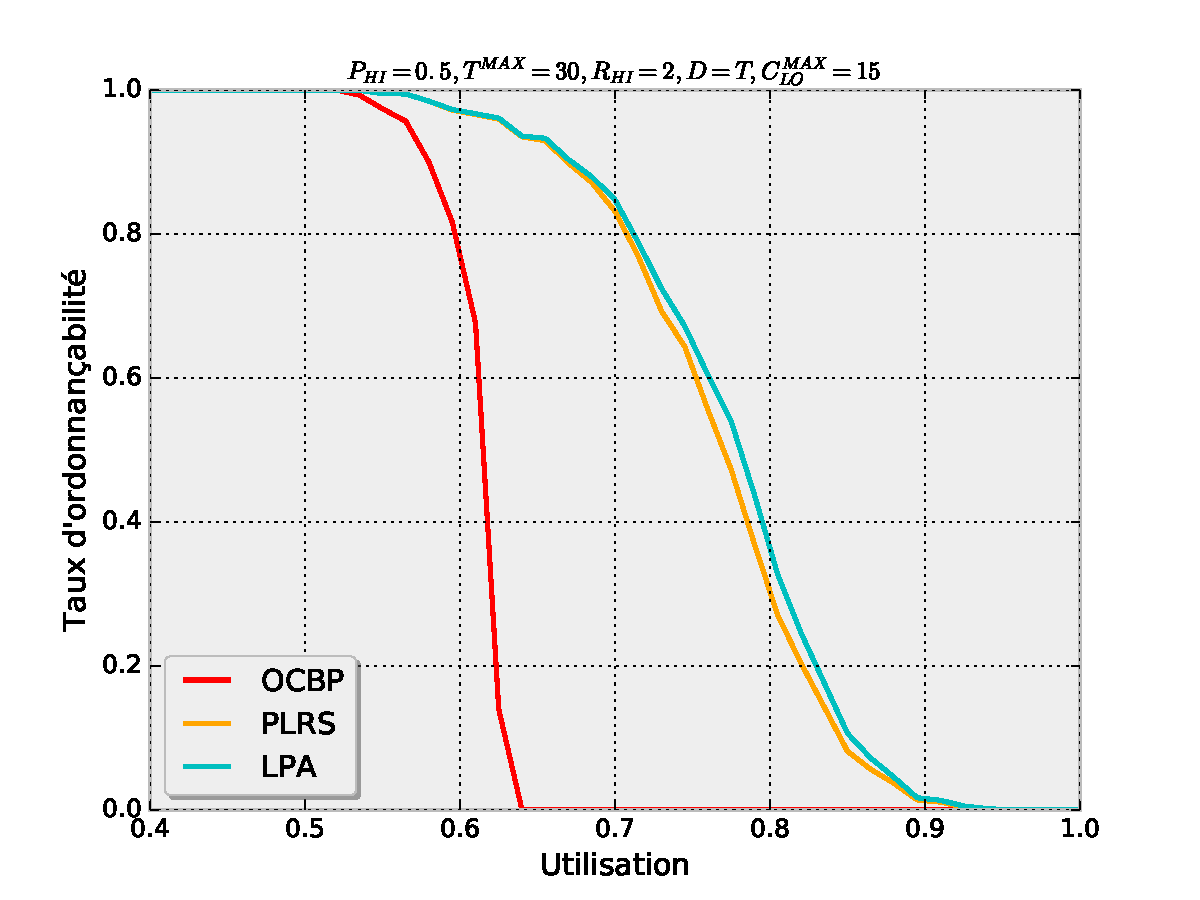
\includegraphics[width=\textwidth,height=0.8\textheight,keepaspectratio]{./results/perfOCBPetc.pdf}
\caption{Ordonnançabilité de OCBP et extensions}
\label{res:ocbpbext}
\end{figure}
\end{frame}


\begin{frame}{EDF-VD}
\begin{figure}[h]
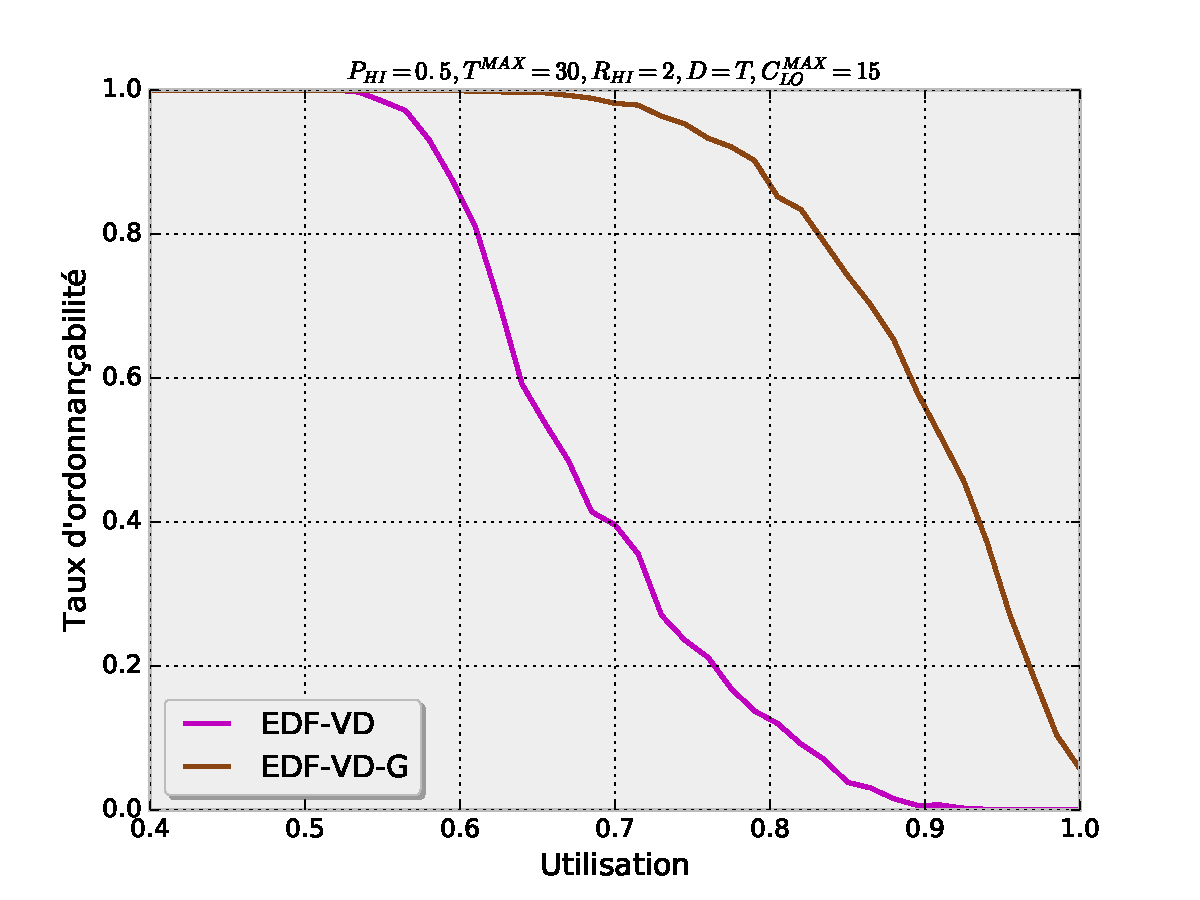
\includegraphics[width=\textwidth,height=0.8\textheight,keepaspectratio]{./results/perfEDFVD.pdf}
\caption{Ordonnançabilité de EDF-VD}
\label{res:edfvd}
\end{figure}
\end{frame}


\begin{frame}{Comparaison}
\begin{figure}[h]
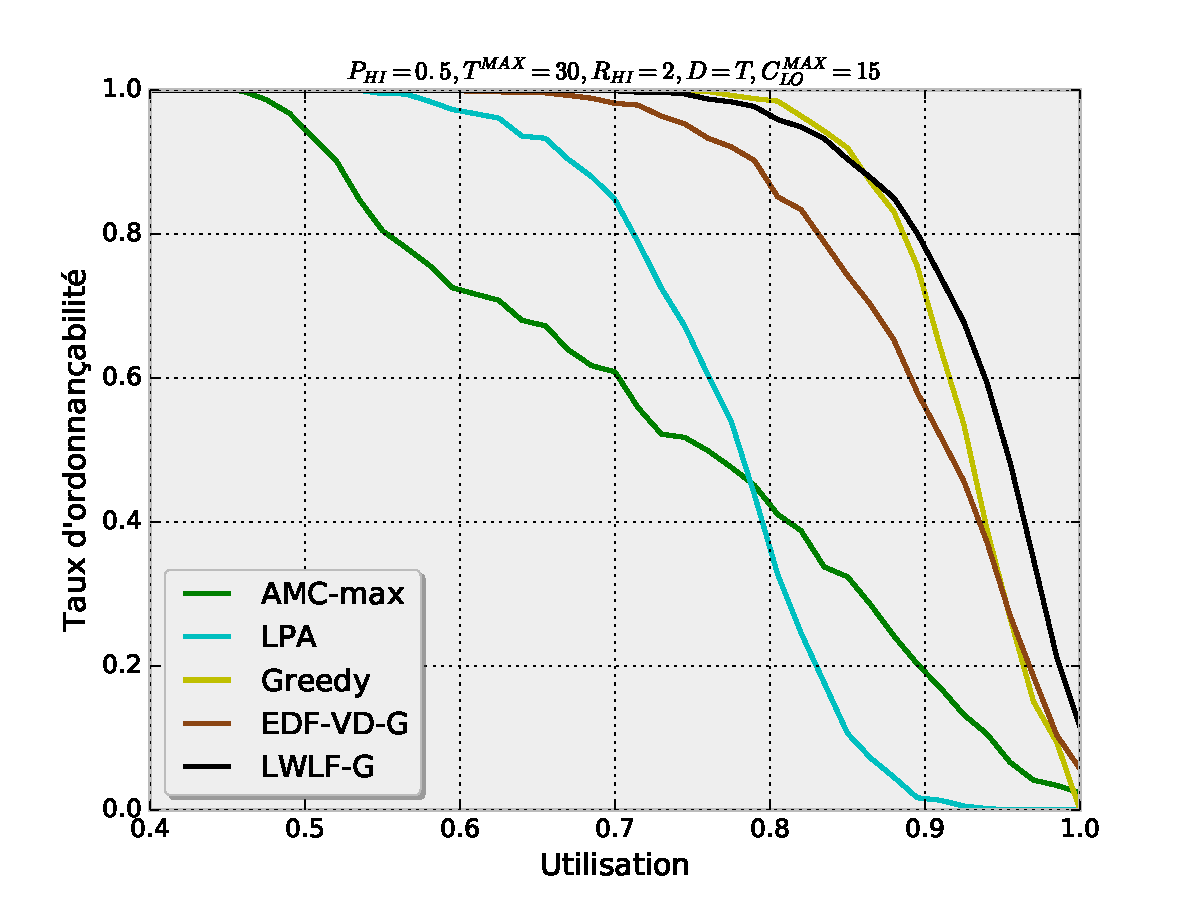
\includegraphics[width=\textwidth,height=0.8\textheight,keepaspectratio]{./results/perfComp.pdf}
\caption{Comparaison des algorithmes}
\label{res:full}
\end{figure}
\end{frame}


\section{Conclusion}


\begin{frame}{Conclusion}

\begin{itemize}
\item Définition de l'ordonnancement en criticité mixte.
\item Présentation d'une réduction vers l'accessibilité
\item Explication de la notions d'antichaînes
\item Regroupement d'algorithme d'ordonnancement CM
\item Proposition de l'algorithme LWLF
\item Test d'ordonnançabilité par explorations d'automate \begin{itemize}
\item Pour système de tâches CM périodique
\item Pour système de tâches CM sporadiques
\item Relation de simulation de tâches oisives
\end{itemize}
\end{itemize}

\begin{itemize}
\item Performance et exportation de la relation de simulation de tâche oisive
\item Démocratisation de l'ordonnancement CM
\item Interdisciplinarité
\item Greedy est un puissant algorithme d'ordonnancement
\item LWLF donne de bon resultats pour des système à haute utilisation
\item Nouvelles possibilités d'exploration de l'ordonnancement CM
\end{itemize}

\end{frame}


\begin{frame}{Travaux ultérieurs}


\begin{itemize}
\item Améliorer l'outil
\item Etendre les tests
\item Explorer de nouvelles relation de simulation
\item Approfondir LWLF
\item Recherche d'un algorithme optimal
\item Jeu d'accèssibilité
\end{itemize}
\end{frame}



\end{document}

